\chapter{Ground Truth: Sockets, Ports, Paths, Users}
Everything in later chapters refers back to this chapter. Memorize the shape, look up the details.

\section{Sockets under \file{/run/kb/}}
\file{/run/kb/} is created by \unit{kbd.service} (\texttt{RuntimeDirectory=kb}, mode 0775) and is
removed by systemd when \cmd{kbd} stops.

\begin{center}
\small
\begin{tabularx}{\textwidth}{@{}L{2.3cm}L{3.3cm}L{2.4cm}Y@{}}
\toprule
\textbf{Socket} & \textbf{Direction} & \textbf{Protocol} & \textbf{Purpose}\\
\midrule
\file{kbd.sock} & \texttt{kbd\_sensor} $\to$ \cmd{kbd} & packed structs & Telemetry only, one direction.\\
\file{kbct.sock} & \cmd{kbd} $\to$ \texttt{kbd\_sensor} & packed structs & Containment and sensitive-path pushes. Split from \file{kbd.sock} so a telemetry burst cannot stall containment.\\
\file{kba.sock} & clients $\to$ \cmd{kbd} & gRPC & Enforcement IPC used by \cmd{kbctl}, \cmd{kbopd}, \cmd{mcp-server}, \cmd{kb-aads}.\\
\file{kbc.sock} & \cmd{kb-checker} diagnostics & gRPC & Watchdog diagnostics (unused while the checker is down).\\
\bottomrule
\end{tabularx}
\end{center}

\section{Network ports}
\begin{center}
\small
\begin{tabularx}{\textwidth}{@{}L{1.6cm}L{3.2cm}L{3.5cm}Y@{}}
\toprule
\textbf{Port} & \textbf{Owner} & \textbf{Bind} & \textbf{Notes}\\
\midrule
8080 & \cmd{kbd} HTTP API + SSE & 127.0.0.1 (flag \texttt{--http-addr}) & REST for processes, alerts, logs, services, metrics, agents, policy; SSE on \texttt{/api/events}. CORS allowlist from \texttt{KB\_HTTP\_CORS\_ORIGIN}.\\
8082 & \cmd{kbopd} embedded dashboard & 127.0.0.1, fixed in the binary & Static Vite app plus \texttt{POST /api/containment}.\\
2222 & operator \cmd{sshd} & all interfaces (\texttt{sshd@kb-operator}) & Key-only console that forces the TUI wrapper.\\
8601 & \cmd{kb-aads} status server & 127.0.0.1 (\file{KB_AADS_STATUS_HOST/PORT}) & Agent status; \cmd{kbd} proxies it for \texttt{/api/agents}.\\
\bottomrule
\end{tabularx}
\end{center}
\begin{kbwarn}[PORT 2222 IS THE ONLY NON-LOOPBACK LISTENER]
The dashboard and API bind loopback on purpose. Remote humans reach the system through SSH on 2222
(Chapter~\ref{ch:ssh}) rather than by exposing HTTP. Keep it that way unless you also set
\texttt{KB\_HTTP\_API\_TOKEN} and a TLS-terminating proxy.
\end{kbwarn}

\section{Filesystem layout after install}
\begin{figure}[ht]
\centering
\small
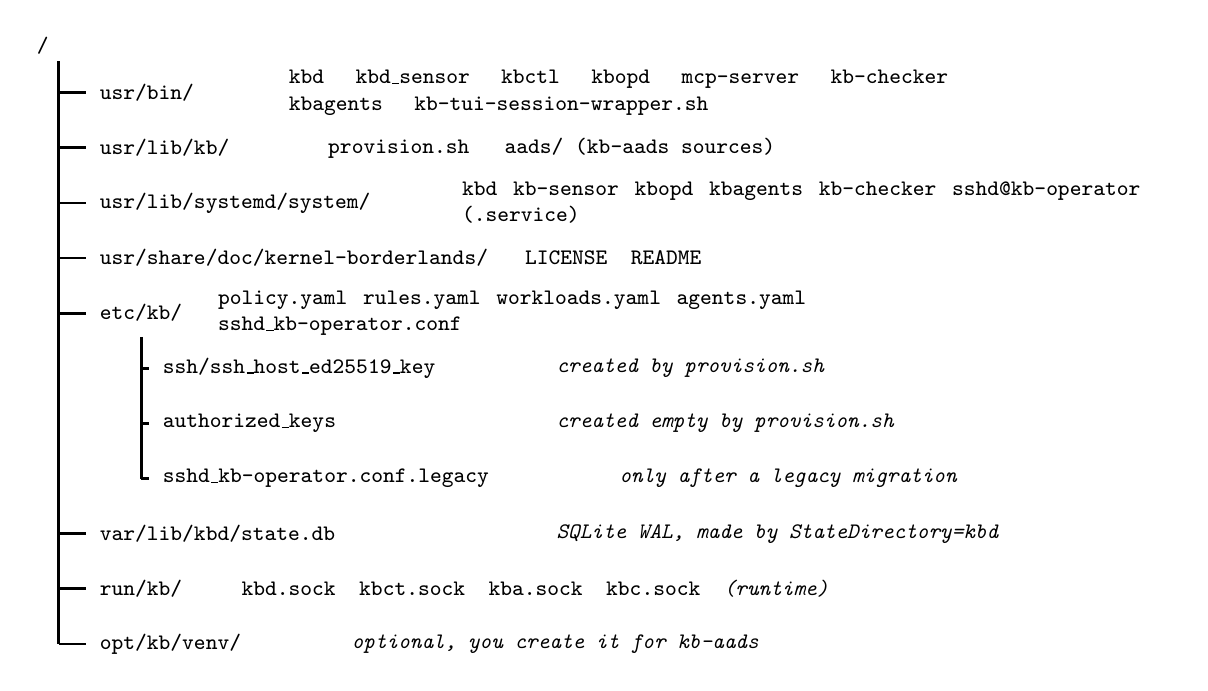
\begin{tikzpicture}[x=1cm,y=1cm]
\tikzset{t/.style={font=\ttfamily\bfseries\footnotesize,anchor=west}}
\node[t] at (0,0) {/};
\node[t] at (0.8,-0.6) {usr/bin/};
\node[t,text width=9cm] at (3.2,-0.6) {kbd \quad kbd\_sensor \quad kbctl \quad kbopd \quad mcp-server \quad kb-checker \quad kbagents \quad kb-tui-session-wrapper.sh};
\node[t] at (0.8,-1.3) {usr/lib/kb/};
\node[t] at (3.7,-1.3) {provision.sh \quad aads/ (kb-aads sources)};
\node[t] at (0.8,-2.0) {usr/lib/systemd/system/};
\node[t,text width=9cm] at (5.4,-2.0) {kbd \ kb-sensor \ kbopd \ kbagents \ kb-checker \ sshd@kb-operator (.service)};
\node[t] at (0.8,-2.7) {usr/share/doc/kernel-borderlands/};
\node[t] at (6.2,-2.7) {LICENSE \ README};
\node[t] at (0.8,-3.4) {etc/kb/};
\node[t,text width=10cm] at (2.3,-3.4) {policy.yaml \ rules.yaml \ workloads.yaml \ agents.yaml \ sshd\_kb-operator.conf};
\node[t] at (1.6,-4.1) {ssh/ssh\_host\_ed25519\_key};
\node[t] at (6.6,-4.1) {\textit{created by provision.sh}};
\node[t] at (1.6,-4.8) {authorized\_keys};
\node[t] at (6.6,-4.8) {\textit{created empty by provision.sh}};
\node[t] at (1.6,-5.5) {sshd\_kb-operator.conf.legacy};
\node[t] at (7.4,-5.5) {\textit{only after a legacy migration}};
\node[t] at (0.8,-6.2) {var/lib/kbd/state.db};
\node[t] at (6.6,-6.2) {\textit{SQLite WAL, made by StateDirectory=kbd}};
\node[t] at (0.8,-6.9) {run/kb/};
\node[t] at (2.6,-6.9) {kbd.sock \ kbct.sock \ kba.sock \ kbc.sock \ \textit{(runtime)}};
\node[t] at (0.8,-7.6) {opt/kb/venv/};
\node[t] at (4.0,-7.6) {\textit{optional, you create it for kb-aads}};
\draw[line width=1pt] (0.4,-0.2) -- (0.4,-7.6);
\foreach \y in {-0.6,-1.3,-2.0,-2.7,-3.4,-6.2,-6.9,-7.6} \draw[line width=1pt] (0.4,\y) -- (0.75,\y);
\draw[line width=1pt] (1.45,-3.7) -- (1.45,-5.5);
\foreach \y in {-4.1,-4.8,-5.5} \draw[line width=1pt] (1.45,\y) -- (1.55,\y);
\end{tikzpicture}
\caption{Where everything lands. Paths are identical on both distributions.}
\end{figure}

\section{Users, groups, and permissions}
\file{provision.sh} runs from the package's post-install step and is idempotent.
\begin{center}
\small
\begin{tabularx}{\textwidth}{@{}L{3.2cm}Y@{}}
\toprule
\textbf{Object} & \textbf{Definition}\\
\midrule
group \texttt{kb} & System group; owns \file{/etc/kb} (mode 0750, \texttt{root:kb}).\\
user \texttt{operator} & System user, no home, member of \texttt{kb}. The only account the operator \cmd{sshd} accepts (\texttt{Match User operator}).\\
\file{/etc/kb/ssh/ssh_host_ed25519_key} & Host key for the operator \cmd{sshd}, generated on first install, never overwritten.\\
\file{/etc/kb/authorized_keys} & Empty at install, \texttt{operator:kb}, mode 0600. Fill it with \cmd{kbctl ssh add-key}.\\
Config files in \file{/etc/kb} & Mode 0640 root-owned; \cmd{kbd} runs as root. Listed as package conffiles so your edits survive upgrades.\\
\bottomrule
\end{tabularx}
\end{center}

\section{Environment variables}
\begin{center}
\small
\begin{tabularx}{\textwidth}{@{}L{4.6cm}L{3.6cm}Y@{}}
\toprule
\textbf{Variable} & \textbf{Read by} & \textbf{Meaning}\\
\midrule
\texttt{KB\_HTTP\_CORS\_ORIGIN} & \cmd{kbd} & Comma-separated browser origins allowed to call the API. The packaged unit sets \texttt{http://127.0.0.1:8082,http://localhost:8082}. Default without it: the Vite dev origins on 5173 only.\\
\texttt{KB\_HTTP\_API\_TOKEN} & \cmd{kbd} & Bearer token gating the mutating routes (\texttt{isolate}, \texttt{restore}). Unset means those routes fail closed.\\
\texttt{KB\_AADS\_STATUS\_HOST}, \texttt{KB\_AADS\_STATUS\_PORT} & \cmd{kbagents} & Bind address of the agent status server (default 127.0.0.1:8601).\\
\texttt{KB\_AADS\_API\_ADDR} & \cmd{kbd} & Where \cmd{kbd} proxies \texttt{/api/agents}; must match the status server.\\
\bottomrule
\end{tabularx}
\end{center}
